\section{Literature Review}\label{sect:litreview}

The use of Genetic Algorithms (GAs) for solving optimization problems is a well-established research area.
The first GA was proposed by Holland in 1975~\cite{holland1975adaptation} and it was based on the principles of natural selection and evolution.
The GA is a metaheuristic that is inspired by the biological evolution process and it is used to find optimal solutions to optimization problems.
It is also a stochastic population based algorithm that uses a population of candidate solutions to find the optimal solution. It is not guaranteed
to find a global optimum, but it is likely to find an acceptable solution that may be close to the global optimum.~\cite{alba2008introduction}

In the scope of optimizing resource allocation, GAs have been used to solve a plethora of problems. In the latest decades, the constant improvement and implementation
of the various parts of genetic algorithms, in particular on the crossover function, helped to improve the performances of GAs in the scheduling and
assignation of resources.~\cite{alcaraz2001robust}

There have been many comparisons between GAs and other metaheuristics, such as Simulated Annealing (SA) and Tabu Search (TS).
Not only under the aspect of resource allocation, but also in their effectiveness in solving other optimization problems.~\cite{vasan2009comparative, ross1995comparing}
It is worth mentioning that they can be used in combination with \textit{Machine Learning} techniques, such as \textit{Neural Networks}, to improve the quality of the training
of many models and architectures.~\cite{sexton1999optimization}

The main difference between GAs and SA is that GAs are population based algorithms, while SA is a single solution based algorithm. The scope of the research
drifted towards the comparison between GAs and TS, which is a memory based algorithm~\cite{zolfaghari2002comparative, youssef2001evolutionary} at first, then it shifted mostly
towards the comparison between GAs and Particle Swarm Optimization.~\cite{hassan2005comparison}

From the point of view of using genetic algorithms for optimizing different aspects of cloud computing environments, the literature is rich and diverse.
Let's take as example task scheduling, which is an NP-complex problem. It is clear that it possesses a key role in cloud computing systems.
The paper from $2009$ written by Chenhong et al.~\cite{5301850} explores various genetic algorithm for task scheduling in cloud computing environments and takes into account 
the divisibility of the tasks that adapt to different computation and memory requirements. So, the system is treated as an heterogeneous system. 
The interesting part is that at the time, Genetic Algorithms were deemed unfit to solve global optimization problems and had to be optimized further.~\cite{5301850}

It is in $2011$ that Zhu et al. proposed a new genetic algorithm for task scheduling in cloud computing environments.
By proposing a Multi-Agent genetic algorithm, called \textit{MAGA}, the authors were capable of surpassing the performances of the traditional GA.
It was used mostly to solve load balancing problems in cloud computing. It is worth mentioning that \textit{MAGA} proved itself to be even more effective than the 
\textit{Min-Max Strategy}.~\cite{zhu2011genetic} 
The \textit{Min-Max Strategy}, on the other hand, is a road that was abandoned as a standalone solution in cloud computing environments when compared to Genetic Algorithms. In fact it
was studied to be incorporated in more complex ones.~\cite{elzeki2012improved}

To follow, an extensive literature review of the last decade highlitghts the most relevant papers in the field of artificial intelligence applied to
cloud computing and genetic algorithms, winth particular regard to Genetic Algorithms and other meta heuristics such as Particle Swarm Optimization.

\subsection{Hybrid Genetic Algorithm for Cloud Computing Applications by Zhu et al.}
This paper, written in $2011$, is one of the first and most relevant papers in the field of genetic algorithms for resource allocation
in cloud computing. The idea behind this research was to produce an hybrid GA capable of performing better than a classic one.
The algorithm proposed was called \textit{MAGA} and it was implemented by treating an individual in the GA itself as an agent, capable 
of local perception, competition, cooperation and self improvement towards the puropse of global optimization.
Each agent was capable of exchanging information with its neighbors to achieve these features.

% Insert a centered image here
\begin{figure}[h]
    \centering
    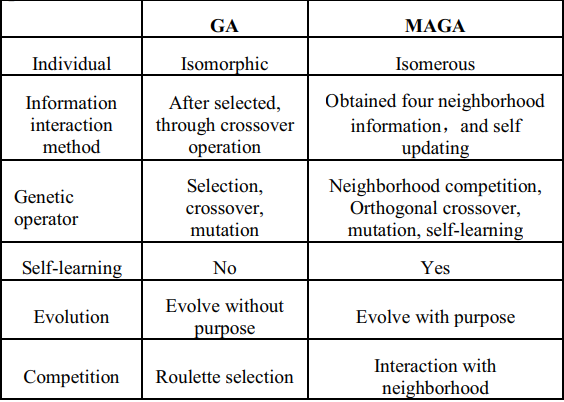
\includegraphics[width=0.5\textwidth]{Resources/litreview/MAGA/ga_vs_maga.png}
    \caption{The main differences between the classic GA and the MAGA.}
    \label{table:maga}
\end{figure}

As is shown in Table~\ref{table:maga}, the differences outlined are quite evident.
There are also some heavby differences in the genetic operators.
In \textit{MAGA} they include \textit{neighborhood competition operator}, \textit{neighborhood orthogonal crossover operator}, 
\textit{mutation operator}, and the \textit{self-learning operator}.
The first one is responsible for the competition among the agents, while the second one achieves collaboration between them. 
Mutation and Self-learning oeprators allow the agents to use their knowledge.
In conclusion, the authors developed an algorithm that experimentally proved the superiority of the MAGA over the classic GA when handling high-dimensional optimization problems.
The paper also presented a cloud computing load balancing model and applied the MAGA algorithm for resource scheduling, demonstrating that MAGA performs way better even than
the \textit{Min-Min} scheduling algorithm.~\cite{zhu2011genetic}

\subsection{A New Resource Scheduling Strategy Based on Genetic Algorithm in Cloud Computing Environment by Gu et al.}
This paper proposes a load balancing strategy for virtual machine (VM) resources scheduling in cloud computing based on genetic algorithms. 
The aim of this strategy is to achieve the best load balancing while reducing or avoiding dynamic migration, 
thus resolving the problem of load unbalancing and high migration costs. 
The proposed algorithm computes in advance the influence it will have on the system after the deployment of the needed VM resources, 
and then chooses the least-affective solution. 
The method considers historical data and current states of the system and uses a tree structure for genetic algorithm coding. 
The selection, hybridization, and variation strategies are also proposed to improve the algorithm's performance.

To evaluate the proposed method, the authors introduced a variation rate to describe the load variation of system virtual machines and used the average load distance 
to measure the overall load balancing effect of the algorithm. Experimental results showed that the proposed method has fairly good global astringency and efficiency, 
and it can better realize load balancing and proper resource utilization.

While the proposed algorithm has shown promising results, it has some limitations. 
In real cloud computing environments, there might be dynamic changes in VMs and an increase in computing cost of virtualization software, 
leading to unpredicted load wastage with the increase of VM number started on every physical machine. 
Therefore, a monitoring and analyzing mechanism is needed to better solve the problem of load balancing, which is also a further research subject.~\cite{gu2012new}

\subsection{Load Balancing Task Scheduling Based on Genetic Algorithm in Cloud Computing by Tingting et al.}

Task scheduling is one of the most critical issues in cloud computing environments due to the huge number of users and tremendous data volume. 
Efficient task scheduling mechanisms should meet users' requirements and improve resource utilization to enhance the overall performance of the cloud platform. 
To solve this problem, this paper proposes a new scheduling algorithm based on the double-fitness adaptive algorithm 
(job spanning time and load balancing genetic algorithm (JLGA)) that considers the new characteristics of cloud computing and the original adaptive genetic algorithm (AGA).~\cite{jakobovic1999adaptive}
The proposed algorithm not only works out a task scheduling sequence with shorter job and average job makespan but also satisfies inter-nodes load balancing.

To improve the performance of the algorithm, this paper adopts a greedy algorithm to initialize the population, introduces variance to describe the load intensity among nodes, 
and weights the multi-fitness function. The paper experimentally evaluates the performance of the JLGA algorithm and the DGA with 30 jobs. 

% Insert two centered images in the same figure here

\begin{figure}[!htb]
    \begin{minipage}{0.48\textwidth}
      \centering
      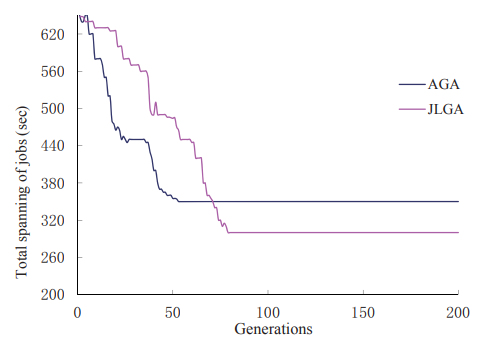
\includegraphics[width=1\textwidth]{Resources/litreview/MAGA/aga_vs_jlga_2.png}
      \caption{Total spanning of jobs}\label{Fig:jlga1}
    \end{minipage}\hfill
    \begin{minipage}{0.48\textwidth}
      \centering
      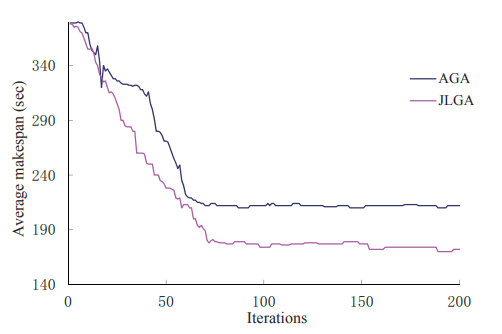
\includegraphics[width=1\textwidth]{Resources/litreview/MAGA/aga_vs_jlga_1.png}
      \caption{Average spanning of jobs}\label{Fig:jlga2}
    \end{minipage}
 \end{figure}


The results in Figure~\ref{Fig:jlga1} and in Fifgure~\ref{Fig:jlga2} show that JLGA takes little time both in total job and average job consuming, 
and it balances the entire system load effectively.

However, there are two interesting points that deserve further investigation. Firstly, in real cloud computing environments, job priorities cannot be avoided. 
Secondly, other static parameters in GA, such as population scale, iterations, crossover, and mutation operator, may put pressure on the speed of convergence and 
quality of global optimal solution. Therefore, another further research subject may consider a dynamic global adaptive control strategy in the genetic algorithm. 
For example, population scale should be large in the early generations to maintain diversity and decrease to converge rapidly during the latter generations. 
Individuals with better performance should cross more while lower fitness individuals should mutate to adapt to the fitness function. 
Considering the particularity of the cloud environment, the time complexity should not be too high.~\cite{wang2014load}

\newpage
